\documentclass[11pt]{report}
\usepackage{eso-pic,graphicx}
\usepackage[export]{adjustbox}
\usepackage{url}
\usepackage[top=2cm, bottom=2cm, outer=2cm, inner=2cm]{geometry}
\begin{document}
%\AddToShipoutPictureBG*{
\includegraphics[width=\paperwidth,height=\paperheight]{images/bkgrnd}}
\begin{center}
\vspace*{2cm}
\textsf{\begin{Huge}
\textbf{ELP­718 ­ Telecom Software Laboratory \\
1st Semester, 2016-18 \\
Abhishek Mishra\\
8 Nov 2016, 5pm\\
Assignment-13}\\
\end{Huge}}
\vspace*{6cm}

\includegraphics[scale=0.12, center]{images/iitlogo}
\end{center}
\pagebreak
\tableofcontents
\vspace{5cm}
\pagebreak
\section{Problem Statement 1}
Implement a command-line based URL defragmenter Server using sockets API in C. Develop a client-server based system , where the client sends a URL to the server and the server breaks down the URL into its components and returns them to the client,which displays the result.\\

%	%\begin{figure}[h!]
%	%\centering
%	%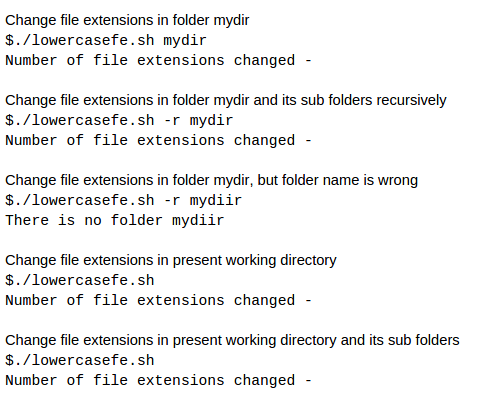
\includegraphics[scale=0.7]{images/Selection_003}	
%	%\end{figure}
\subsection{Assumptions}
Url contains all components.
\subsection{Structure Chart and Implementation}
	\begin{figure}[h!]
	\centering
	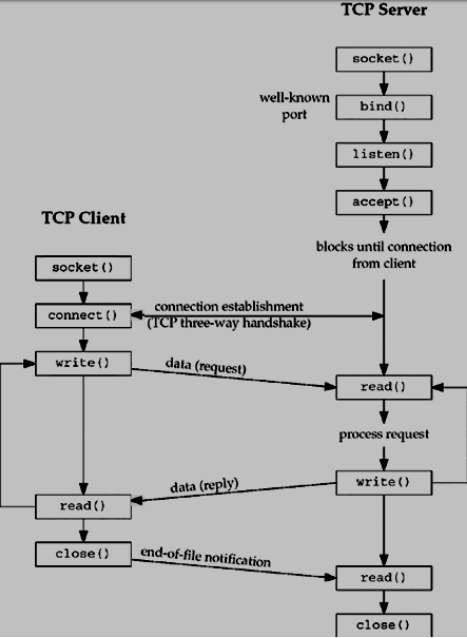
\includegraphics[scale=0.5]{images/sc11}
	\caption{Structure chart for problem 1}
	\end{figure}		
	\pagebreak
	\begin{figure}[h!]
	\centering
	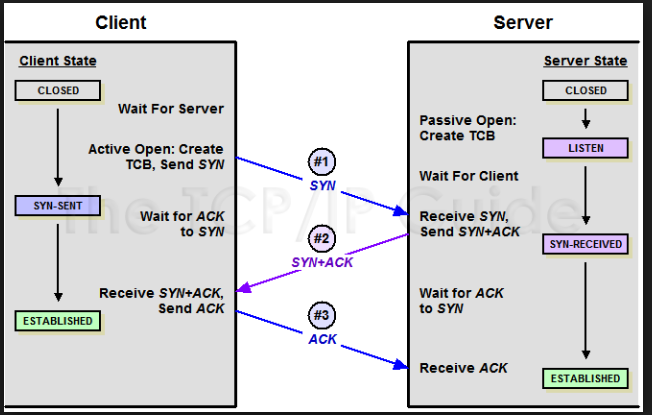
\includegraphics[scale=0.5]{images/sc12}
	\caption{Structure chart for problem 1}
	\end{figure}		
	\pagebreak
\subsection{Screenshots}
	\begin{figure}[h!]
	\centering
	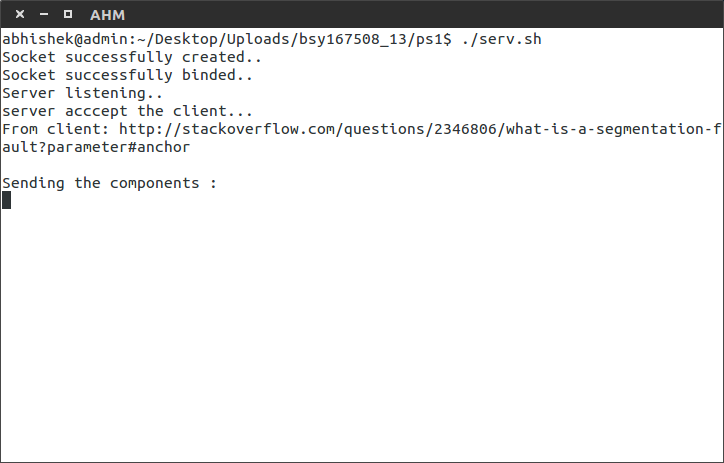
\includegraphics[scale=0.8, center]{images/screenshot11}
	\caption{Screenshot for problem statement 1}
	\end{figure}
	\begin{figure}[h!]
	\centering
	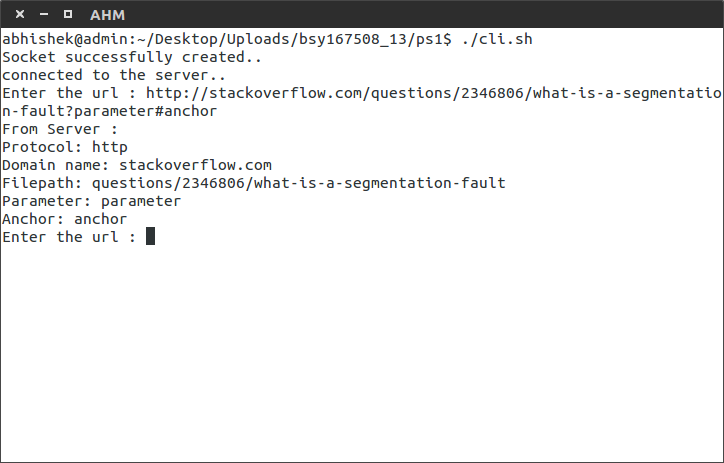
\includegraphics[scale=0.8, center]{images/screenshot12}
	\caption{Screenshot for problem statement 1}
	\end{figure}
	\pagebreak
%	%\iffalse
\section{Problem Statement 2}
Implement a client - server model based DHCP server functionality simulator using sockets API in C.The Server application has to support at least five clients simultaneously.\\
\subsection{Assumptions}
Each client has unique mac address. There are maximum 5 clients.
\pagebreak
\subsection{Structure Chart}
	\begin{figure}[h!]
	\centering
	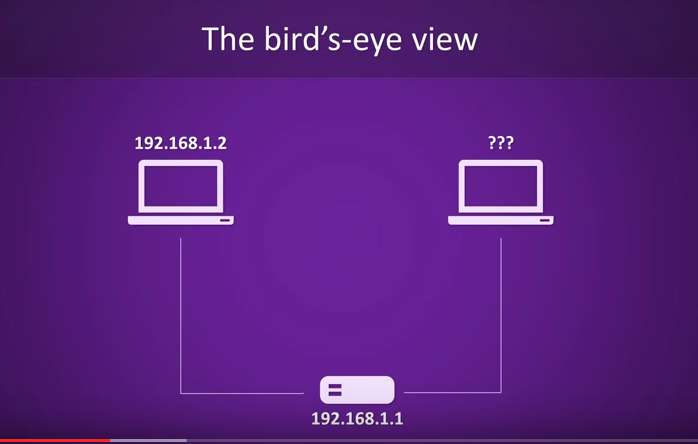
\includegraphics[scale=0.7]{images/sc21}
	\caption{Structure chart for problem 2  }	
	\end{figure}
	\pagebreak
	\begin{figure}[h!]
	\centering
	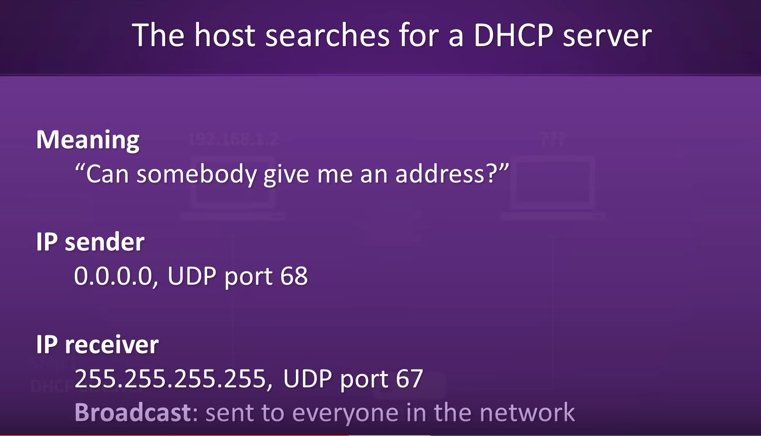
\includegraphics[scale=0.7]{images/sc22}
	\caption{Structure chart for problem 2 }	
	\end{figure}
	\pagebreak
	\begin{figure}[h!]
	\centering
	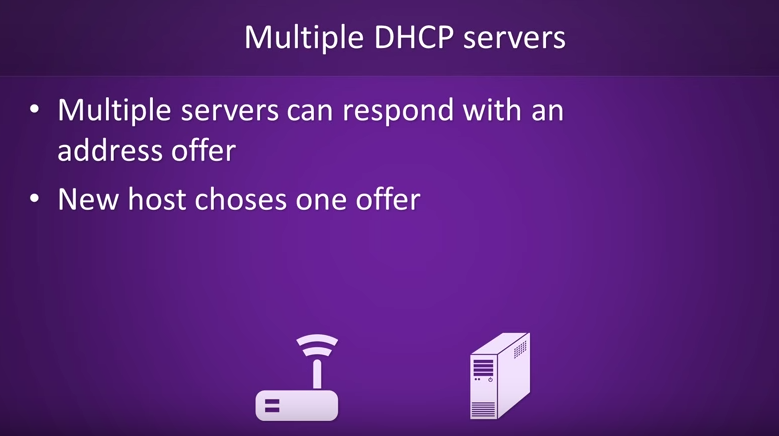
\includegraphics[scale=0.7]{images/sc23}
	\caption{Structure chart for problem 2 }	
	\end{figure}
	\pagebreak
	\begin{figure}[h!]
	\centering
	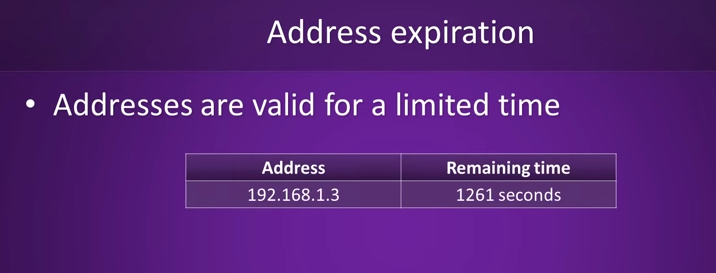
\includegraphics[scale=0.7]{images/sc24}
	\caption{Structure chart for problem 2 }	
	\end{figure}
	\pagebreak
\subsection{Screenshots}
	\begin{figure}[h!]
	\centering
	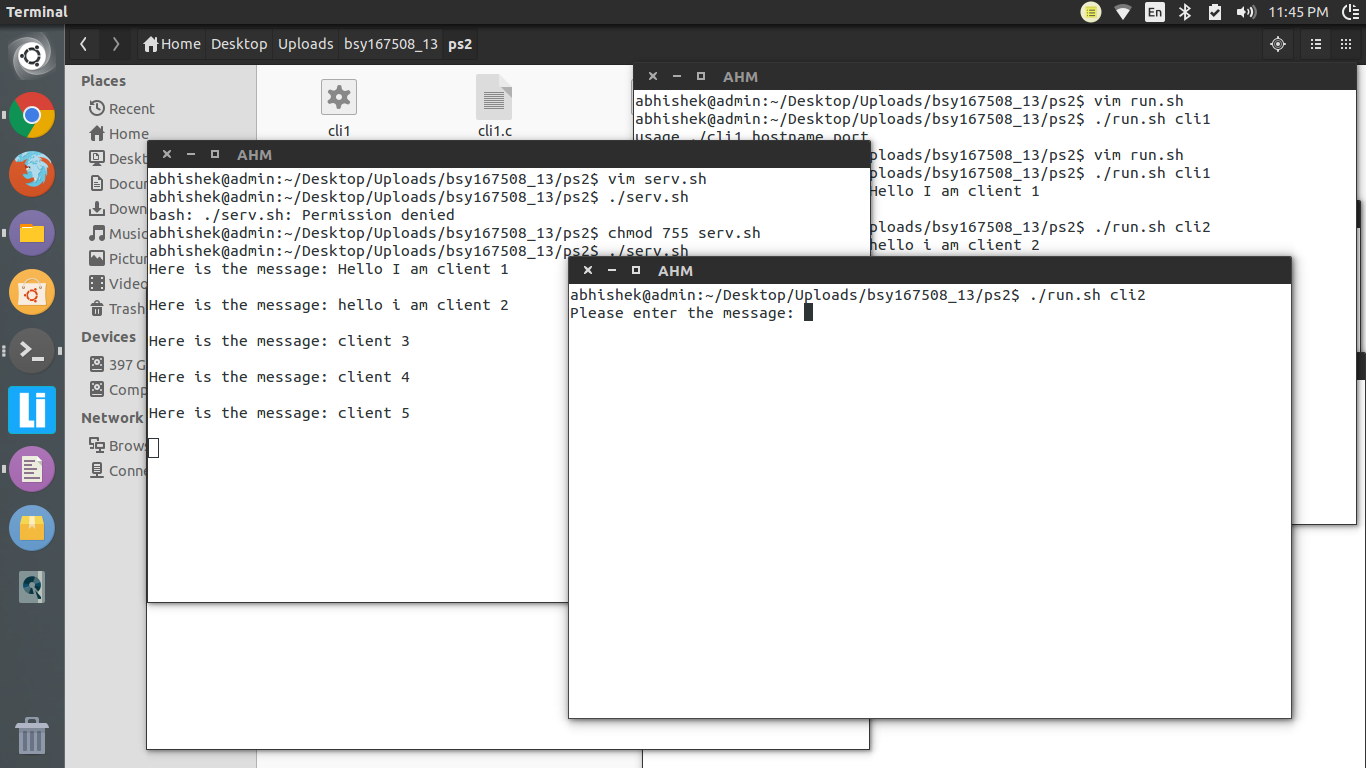
\includegraphics[scale=0.8, center]{images/screenshot21}
	\caption{Screenshot for problem statement 2}
	\end{figure}
	\pagebreak
%	\begin{figure}[h!]
%	\centering
%	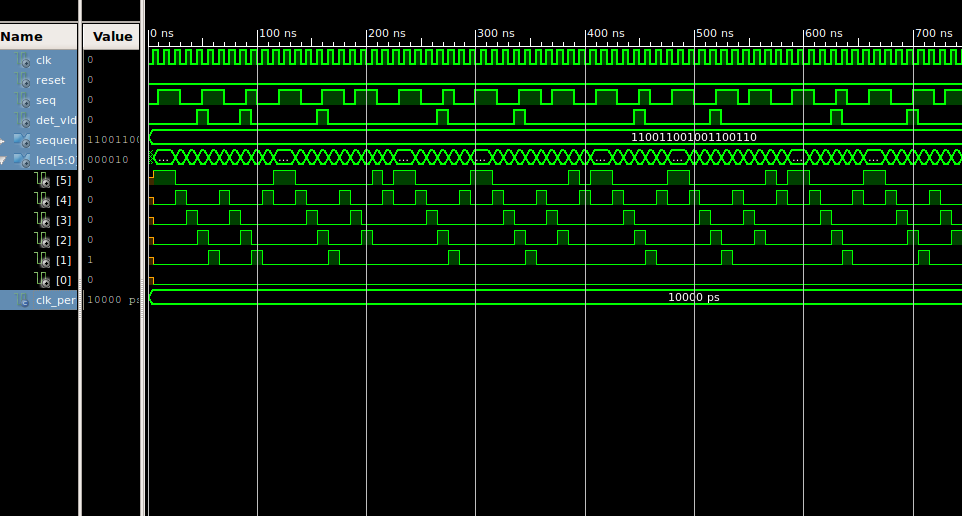
\includegraphics[scale=0.8, center]{images/screenshot22}
%	\caption{Screenshot for problem statement 2}
%	\end{figure}
%	\pagebreak
%	\begin{figure}[h!]
%	\centering
%	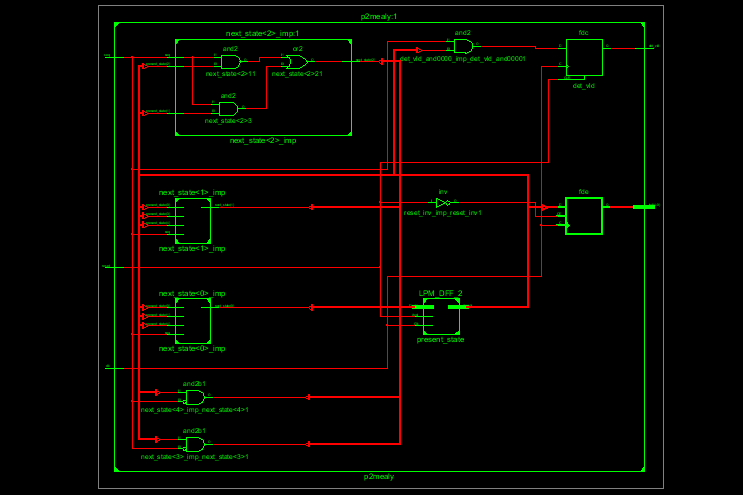
\includegraphics[scale=0.8, center]{images/screenshot23}
%	\caption{Screenshot for problem statement 2}
%	\end{figure}
%	\pagebreak
%	\begin{figure}[h!]
%	\centering
%	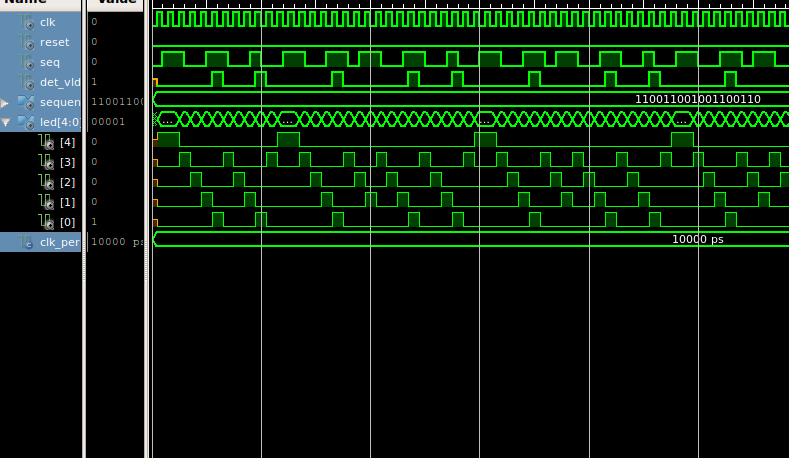
\includegraphics[scale=0.6, center]{images/screenshot24}
%	\caption{Screenshot for problem statement 2}
%	\end{figure}
%	\pagebreak
%	\begin{figure}[h!]
%	\centering
%	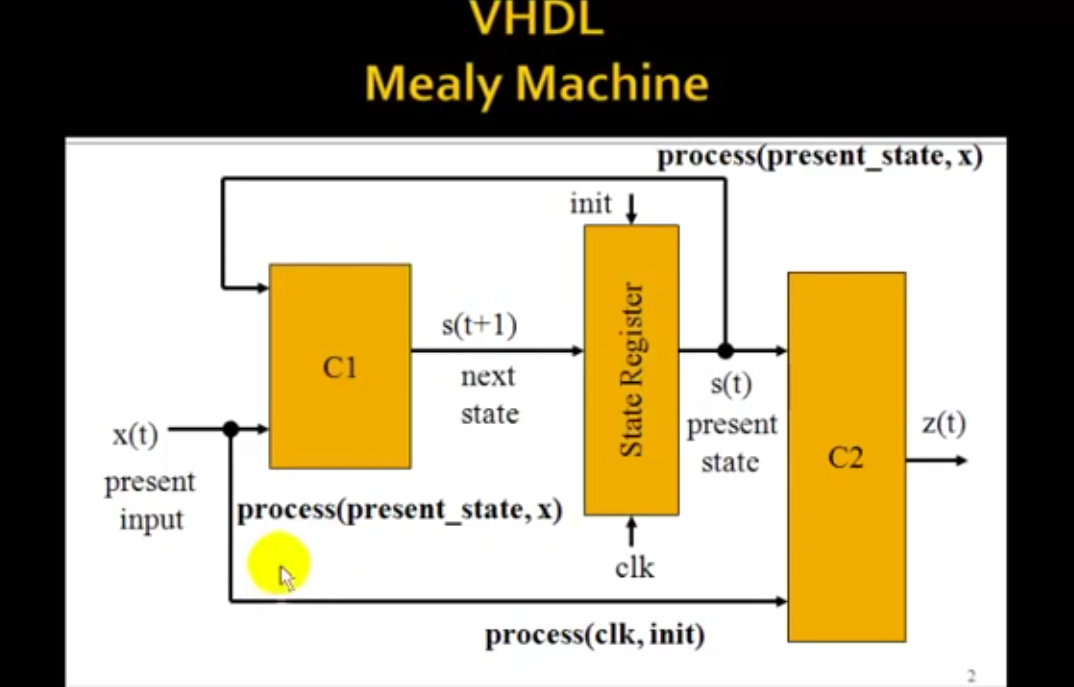
\includegraphics[scale=0.6, center]{images/screenshot25}
%	\caption{Screenshot for problem statement 2}
%	\end{figure}
%	\pagebreak
%	\begin{figure}[h!]
%	\centering
%	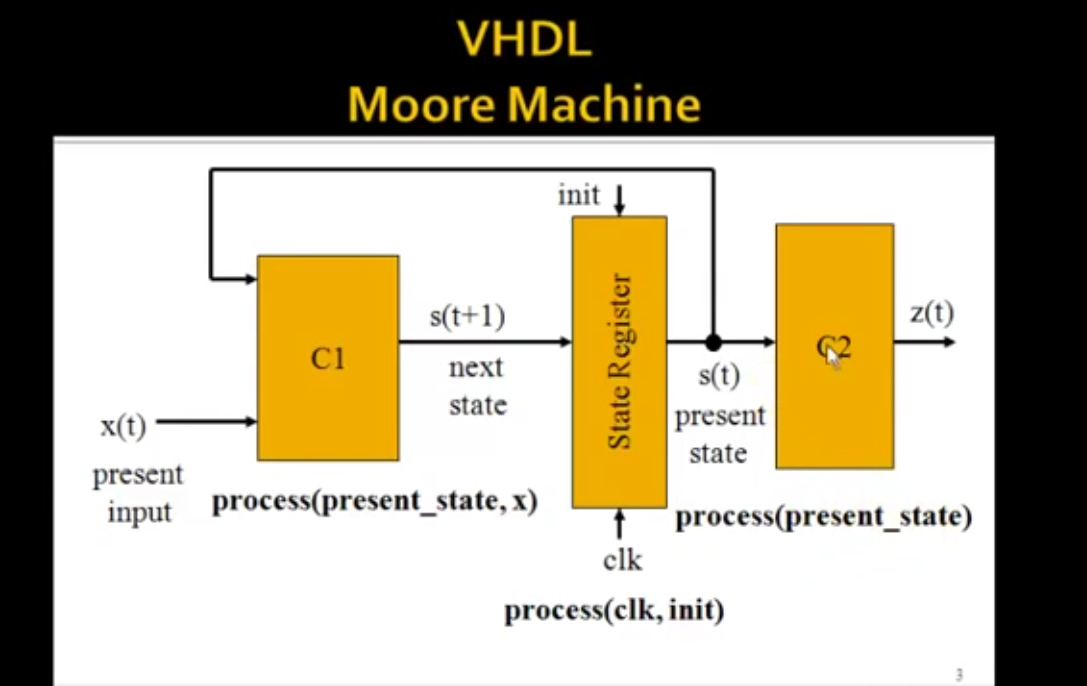
\includegraphics[scale=0.6, center]{images/screenshot26}
%	\caption{Screenshot for problem statement 2}
%	\end{figure}
%	\pagebreak
%\section{Problem Statement 3}
%\textbf{Part - 1 -}\\
%Write shell script to emulate behaviour of bash, but also record every command put up on terminal on a logger.txt file along with time stamp. Your command prompt should look like normal bash command prompt. \\
%	\subsection{Assumptions}
%	The output is to be processed in the exact manner as shown in the image\\
%	\begin{figure}[h!]
%	\centering
%%	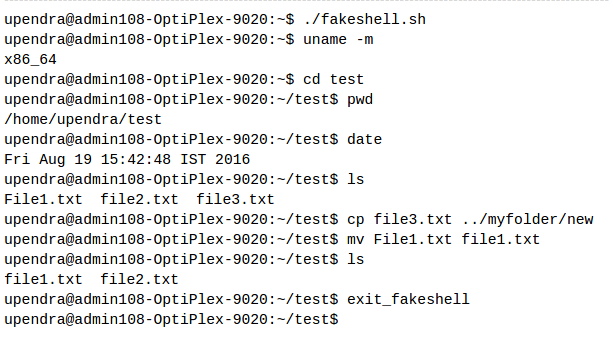
\includegraphics[scale=0.7]{images/Selection_004}	
%	\end{figure}
%	\pagebreak
%	\subsection{Structure Chart}
%	\begin{figure}[h!]
%	\centering
%	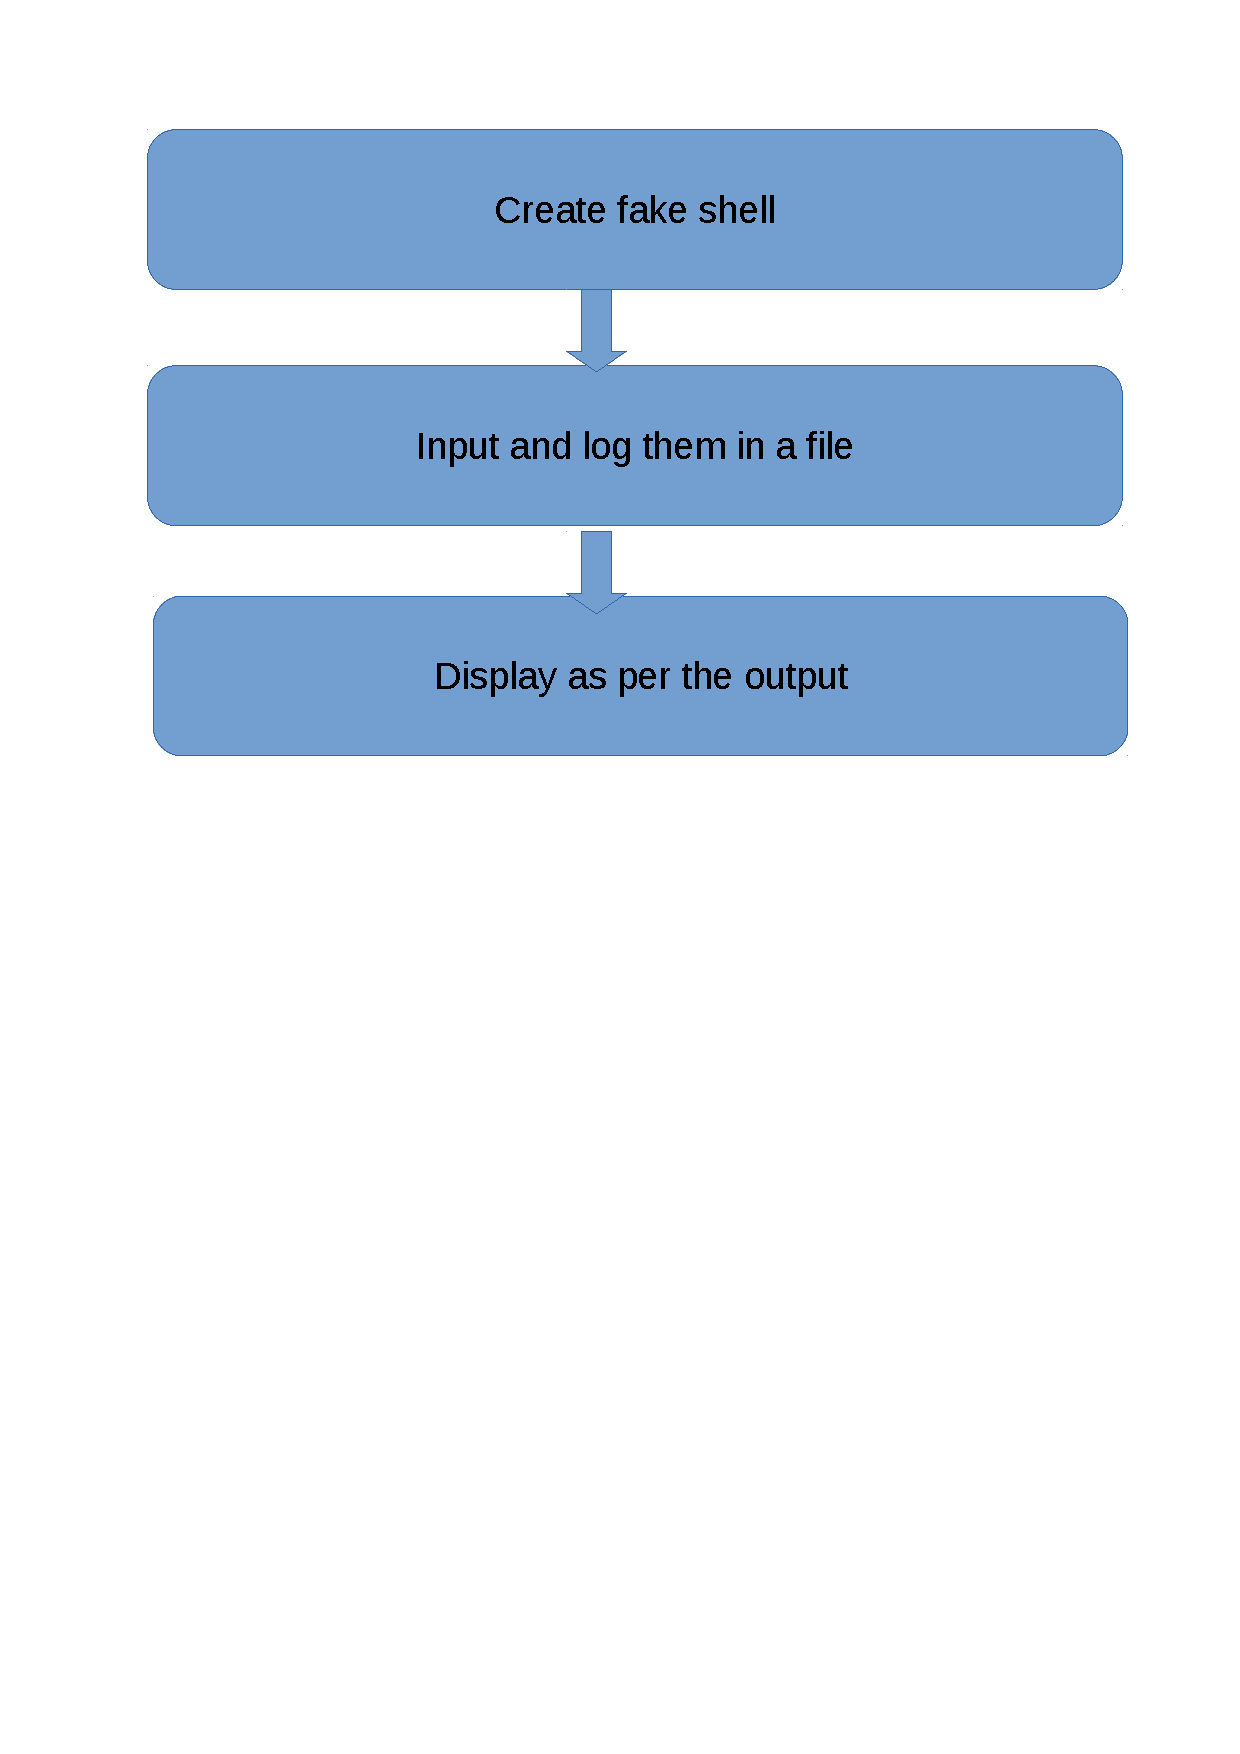
\includegraphics[scale=0.7]{images/shots33}
%	\caption{Structure chart for problem 3}	
%	\end{figure}
%	\pagebreak
%	%\fi
%	\pagebreak
\section{Epilogue}
The first problem statement involved use of tcp server and client systems which can communicate with each other and exchange url and its components.
The second problem involved simulation of dhcp server client relationship. In this we had to show how each gets assigned its ip address.
\bibliography{biblio}
\bibliographystyle{ieeetr}
\nocite{*}
\end{document}